% !TEX root = ../main-ring-signature.tex

Ring signatures, introduced by Rivest, Shamir and Tauman, \cite{AC:RivShaTau01}, allow to anonymously sign a message on behalf of a ring of users $R=\{P_1,\ldots,P_n\}$, only if the signer belongs to that ring. That is, no one outside $R$ can forge a valid signature and  an honestly computed signature reveals (essentially) no information about the actual signer.  
Unlike other similar primitives such as group signatures \cite{EC:ChaVan91}, ring signatures are not coordinated: each user generates secret/public keys on his own --- i.e.~no central authorities --- and might sign on behalf of a ring without the approval or assistance of the other members.

The original motivation for ring signatures was anonymous leakage of secrets. Suppose a high rank officer wants to leak some sensitive information to a journalist without revealing its identity. To do so, it signs this information using a ring signature where the ring contains all other high rank officer. Besides this hypothetical application, with the advent of cryptocurrency ring signatures have found new and more practical applications. For example, for spending a coin in Monero, a user form a ring from public keys in the blockchain to issue a ring signature on the transaction. Thereby, the anonimity properties of the ring signature guarantees untraceability and fungibility. 
Given the practical usefullness of ring signatures, it becomes crucial to study and improve its efficiency.

\subsection{Related Work}
The efficiency of a ring signature might be splitted in three parrameters: the signature size, the cost (time) of computig a signature, and the cost (time) of verifying a signature. Among these metrics, the signature size has received the most attention and improvements in the size ussally imply improvement on the other metrics.
In terms of ring size, the most efficient constructions have signature size logarithmic in the size of the ring \cite{EC:GroKoh15,EC:LLNW16}. However,  both constructions rely on the {random oracle model}, which is an idealization of hash functions and with known inconsitencie \cite{FOCS:GolKal03}. Malavolta et al.~ constructed a constant size ring signature without random oracles \cite{AC:MalSho17}. However, their construction achieves constant-size signatures at the cost of relying on controversial non-falsifiable assumptions \cite{C:Naor03} such as the knowledge of exponent assumption.
Given the disadvantages of random oracles and non-falsifiable assumptions, it is worth to explore constructions from more standard assumptions.

Chase and Lysyanskaya introduced signatures of knowledge \cite{C:ChaLys06} and using this primitive constructed constant-size ring signatures from accumulators, following Dodis et al.\cite{EC:DKNS04}. The scheme description is sparsely detailed and no proof of security is given but, for fairness, we have to say that their work is previous to the formal definition of ring signatures of Bender et al.~\cite{TCC:BenKatMor06}. However, a quick analysis of their proposed scheme shows that is impractical. Their scheme goes as follows.
Given a ring of RSA public keys $R = \{y_1,...,y_n\}\subseteq \Z_{\phi(N)}$, one can compute an accumulated value $a = g^{\prod_{i=1}^n y_i}$ and a witness $w_i = a^{-y_i} \mod N$ that $y_i$ is accumulated in $a$, which can be verified cheking if $a = w_i^{y_i} \mod N$. A ring signature on a message $m$ is computed as a signature on $m$ of knowledge of $x_i,y_i\in \Z_{\phi{N}}, w_i\in \Z_N$ such that: a) $x_iy_i = 1 \mod \phi(N)$ and b)  $a = w_i^{y_i} \mod N$. However, signatures of knowledge are built on top of simulation sound NIZK which in turn is built from normal NIZK. Since no efficient NIZK (without random oracles nor falsifiable assumptions) for statements a) and b) is known, and the only plausible alternative seems generic NIZK arguments for circuit satisfiability, whose proofs are of size $\Omega(|C|)$. For example, using Groth-Sahai proofs, one might expect the circuit for a) and b) to have at least $10^4$ gates, and thus proof will be of size greater than $10^4$ elements of a bilinear group.

Despite Chase and Lysyanskaya's construction, without random oracles nor non-fasifiable assumptions all constructions have signatures of size linear in the size of the ring, being the sole exception the $\Theta(\sqrt{n})$ ring signature of Chandran et al.~\cite{ICALP:ChaGroSah07} 
Although some previous works claim to construct signatures of constant \cite{ACISP:BosDasRan15} or logarithmic \cite{IET:GriSusPla16} size, all of them fail  (see Section \ref{sec:rs-flawed}). The only (non-asymptotic) improvements we are aware of are \cite{TCC:Rafols15,AC:GonHevRaf15}.

\subsection{Our contribution}
In this work we present the first ring signature (without random oracles) whose signature size is asymptotically smaller than Chandran et al.'s. Our ring signature consists of $\Theta(\sqrt[3]{n})$ group elements, computing a signature requires $\Theta(\sqrt[3]{n})$ exponentiations, and verifying a signature requires $\Theta(n^{2/3})$ pairings.

The security of our construction relies on a security assumption --- the {permutation pairing assumption} --- introduced by Groth and Lu \cite{AC:GroLu07} in an unrelated setting: proofs of correctness of a shuffle. While the assumption is ``non-standard'', in the sense that is not a ``DDH like'' assumption, it is a falsifiable assumption and it was proven hard in generic symmetric groups by Groth and Lu. For easiness of exposition, we work on symmetric groups ($\GG_1=\GG_2$) but our techniques might be easily extended to more efficient asymmetric groups in light of recent works on automation of secure symmetric-to-asymmetric conversion \cite{C:AGOT14a,C:AbeHosOhk16,CCS:AkiGarHoh15}.

Our ring signature outperforms Chandran et al.'s in terms signature size for any $n > 144$, in terms of signature generation time for any $n>96$, and in terms of verifier efficiency for any $n>111$. However, this analysis should be taken with care, since Chandran et al.'s signature is proven secure under the decisional linear (DLin) assumption while ours is proven secure under the permutation pairing assumption. Being the permutation pairing assumption much less studied than DLin, it could be the case that our scheme would be as secure as Chandran et al.'s at higher values of the security parameter. In Table \ref{table:eff} we provide a comparison between our scheme and Chandran et al.'s.

\begin{table}[h]
\begin{center}
\begin{minipage}{\textwidth}
\begin{center}
%\begin{scriptsize}
\begin{tabular}{|l|l|l|}
\hline
                                           & Chandran et al.~\cite{ICALP:ChaGroSah07} & This work \\
\hline\hline
\rule{0pt}{2.5ex}CRS size                  & $9$                                       & $9$       \\ 
\rule{0pt}{2.5ex}Verification key size     & $1$                                       & $5$       \\
\rule{0pt}{2.5ex}Signature size            & $24 \sqrt{n} + 24$                        & $39 \sqrt[3]{n} + 30 \sqrt[6]{n} + 81$\\    
\rule{0pt}{2.5ex}Signature generation time & $42 \sqrt{n} + 49$                        & $69 \sqrt[3]{n} + 42 \sqrt[6]{n} + 142$\\
\rule{0pt}{2.5ex}Verification time         & $3 n + 120 \sqrt{n} + 121$                & $6 n^{2/3} + 210 \sqrt[3]{n} + 186 \sqrt[6]{n} + 411$\\
\hline 
\end{tabular}
%\end{scriptsize}
\end{center}
\caption{Comparison of Chandran et al.'s ring signature and ours for a ring of size $n$. 'Signature generation time' is measured in number of exponentiations, 'Verification time' is measured in number of pairings, and all other rows are measured in number of group elements.\label{table:eff}}
\end{minipage}
\end{center}
\end{table}

%
%\begin{figure}[!t]
%	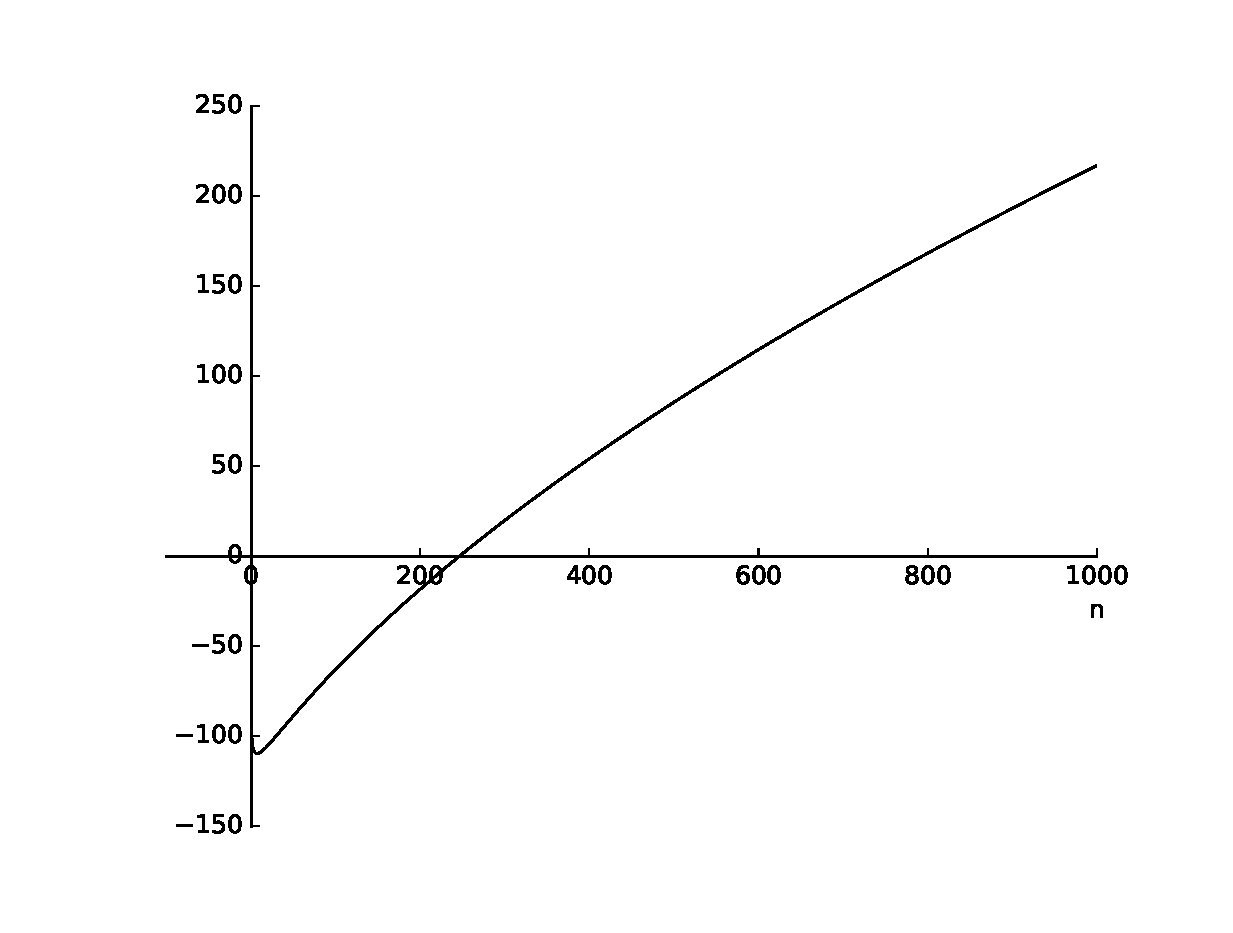
\includegraphics[scale=.25]{intro/sign_size}
%	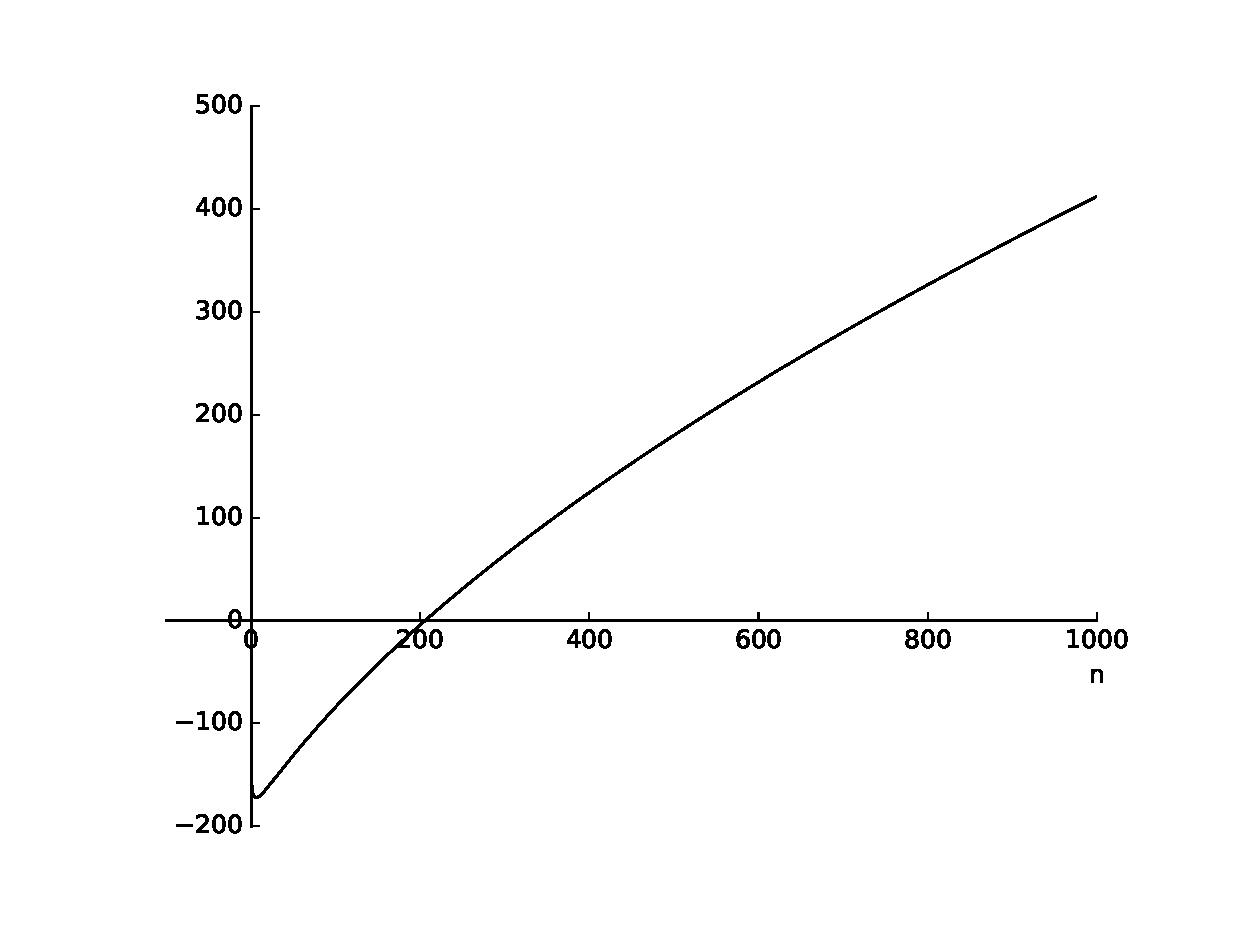
\includegraphics[scale=.25]{intro/sign_time}
%	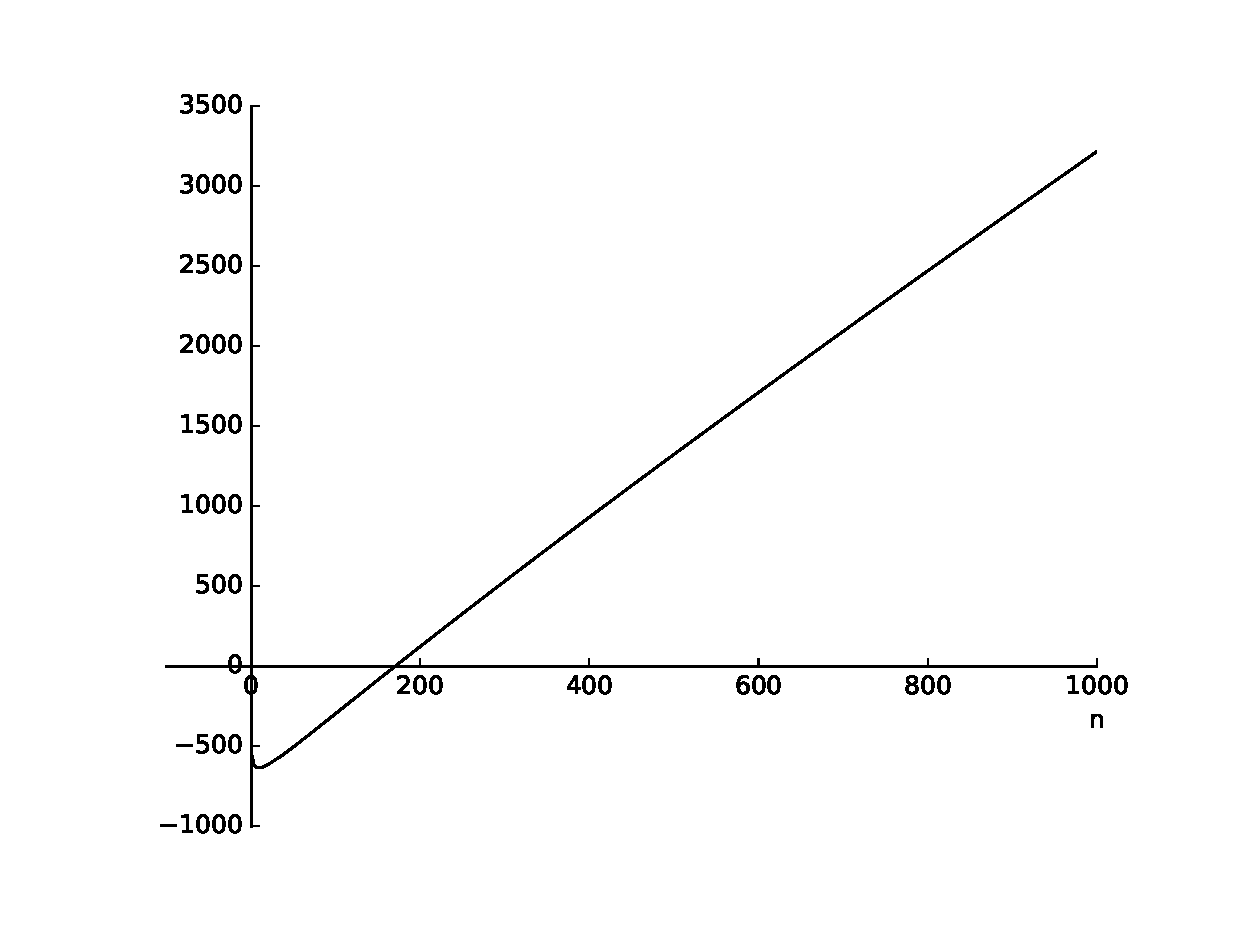
\includegraphics[scale=.25]{intro/ver_time}
%\end{figure}

\subsection{The Hardness of constructing Ring Signatures.}
% !TEX root = ../main-ring-signature.tex

To give a more clear understanding our contributions and to see why other approaches had fail, it will be illustrative what is the main dificuly of constructing a ring signature. Most schemes has followed the following approach: given the set a public keys, sign the message and prove in zero-knowledge that signature can be verified using one of the public keys in the ring. Such statement is known as a 1 out of many proofs.

In general, the diffilculty of proving 1 out of $n$ depends on the nature of the public keys. When they are elements in an field such as the integers one might compute a short digest of the ring, but then is problematic to compute a zero-knowledge proof related to the digest. This is what happens with Chase and Lysyanskaya's and with Bose et al.'s constructions. When  the public keys belong to a less structured group, such as a bilinear group, we don't know how to compute a small digest which is compatible with efficent and expresive NIZK proofs such as Groth-Sahai proofs. Hence, the only step towards was given by Chandran et al.~by reducing the size of the proof from linear to $O(\sqrt{n})$, using techniques from private information retrieval.

Bose et al.~claim to construct a constant-size ring signature in the standard model \cite{ACISP:BosDasRan15}. However, they construct a weak ring signature where: a) the public keys are generated all at once in a correlated way; b) the set of parties which are able to participate in a ring is fixed as well as the maximum ring size; and c) the key size is linear in the maximum ring size. In the work of Chandran et al.~and also in our setting: a) the key generation is independently run by the user using only the CRS as input; b) any party can be member of the ring as long as she has a verification key, and the maximum ring size is unbounded; and c) the key size is constant. These stronger requirements are in line with the original spirit of {non-coordination} of  Rivest et al.~\cite{AC:RivShaTau01}.

Gritti et al.~claim to construct a logarithmic ring signature in the standard model \cite{IET:GriSusPla16}. However, their construction is flawed as explained below.\footnote{We use multiplicative notation for the group operations to keep the expressions as they appear in the original work.}
In page 12, Gritti et al.~define $v_{b_i} := v_{b_1\cdots b_i *}$, where $b_1\cdots b_i *$ is the set of all bit-strings of size $d:=\log n$ whose prefix is $b_1\cdots b_i$. From this, one has to conclude that $v_{b_i}$ is a set (or vector) of group elements of size $2^{d-i}$.
In the same page they define the commitment $D_{b_i} := v_{b_i}h^{s_{b_i}}$, for random $s_{b_i}\in\Z_q$, which, according to the previous observation, is the multiplication of a set (or vector) of group elements with a group element. Given that length reducing group to group commitments are known to not exist \cite{EC:AbeHarOhk12}, its representation requires at least $2^{d-i}$ group elements.\footnote{In fact, there exists length reducing group to group commitments \cite{EC:AKOT15} with a weaker binding property, but is far from clear how to use these commitments in the Gritti et al.'s work} Since commitments $D_{b_0},\ldots,D_{b_d}$ are part of the signature, the actual signature size is $\Theta(2^d)=\Theta(n)$, rather than  $\Theta(d)=\Theta(\log n)$ as claimed by Gritti et al.


